\documentclass[1p]{elsarticle_modified}
%\bibliographystyle{elsarticle-num}

%\usepackage[colorlinks]{hyperref}
%\usepackage{abbrmath_seonhwa} %\Abb, \Ascr, \Acal ,\Abf, \Afrak
\usepackage{amsfonts}
\usepackage{amssymb}
\usepackage{amsmath}
\usepackage{amsthm}
\usepackage{scalefnt}
\usepackage{amsbsy}
\usepackage{kotex}
\usepackage{caption}
\usepackage{subfig}
\usepackage{color}
\usepackage{graphicx}
\usepackage{xcolor} %% white, black, red, green, blue, cyan, magenta, yellow
\usepackage{float}
\usepackage{setspace}
\usepackage{hyperref}

\usepackage{tikz}
\usetikzlibrary{arrows}

\usepackage{multirow}
\usepackage{array} % fixed length table
\usepackage{hhline}

%%%%%%%%%%%%%%%%%%%%%
\makeatletter
\renewcommand*\env@matrix[1][\arraystretch]{%
	\edef\arraystretch{#1}%
	\hskip -\arraycolsep
	\let\@ifnextchar\new@ifnextchar
	\array{*\c@MaxMatrixCols c}}
\makeatother %https://tex.stackexchange.com/questions/14071/how-can-i-increase-the-line-spacing-in-a-matrix
%%%%%%%%%%%%%%%

\usepackage[normalem]{ulem}

\newcommand{\msout}[1]{\ifmmode\text{\sout{\ensuremath{#1}}}\else\sout{#1}\fi}
%SOURCE: \msout is \stkout macro in https://tex.stackexchange.com/questions/20609/strikeout-in-math-mode

\newcommand{\cancel}[1]{
	\ifmmode
	{\color{red}\msout{#1}}
	\else
	{\color{red}\sout{#1}}
	\fi
}

\newcommand{\add}[1]{
	{\color{blue}\uwave{#1}}
}

\newcommand{\replace}[2]{
	\ifmmode
	{\color{red}\msout{#1}}{\color{blue}\uwave{#2}}
	\else
	{\color{red}\sout{#1}}{\color{blue}\uwave{#2}}
	\fi
}

\newcommand{\Sol}{\mathcal{S}} %segment
\newcommand{\D}{D} %diagram
\newcommand{\A}{\mathcal{A}} %arc


%%%%%%%%%%%%%%%%%%%%%%%%%%%%%5 test

\def\sl{\operatorname{\textup{SL}}(2,\Cbb)}
\def\psl{\operatorname{\textup{PSL}}(2,\Cbb)}
\def\quan{\mkern 1mu \triangleright \mkern 1mu}

\theoremstyle{definition}
\newtheorem{thm}{Theorem}[section]
\newtheorem{prop}[thm]{Proposition}
\newtheorem{lem}[thm]{Lemma}
\newtheorem{ques}[thm]{Question}
\newtheorem{cor}[thm]{Corollary}
\newtheorem{defn}[thm]{Definition}
\newtheorem{exam}[thm]{Example}
\newtheorem{rmk}[thm]{Remark}
\newtheorem{alg}[thm]{Algorithm}

\newcommand{\I}{\sqrt{-1}}
\begin{document}

%\begin{frontmatter}
%
%\title{Boundary parabolic representations of knots up to 8 crossings}
%
%%% Group authors per affiliation:
%\author{Yunhi Cho} 
%\address{Department of Mathematics, University of Seoul, Seoul, Korea}
%\ead{yhcho@uos.ac.kr}
%
%
%\author{Seonhwa Kim} %\fnref{s_kim}}
%\address{Center for Geometry and Physics, Institute for Basic Science, Pohang, 37673, Korea}
%\ead{ryeona17@ibs.re.kr}
%
%\author{Hyuk Kim}
%\address{Department of Mathematical Sciences, Seoul National University, Seoul 08826, Korea}
%\ead{hyukkim@snu.ac.kr}
%
%\author{Seokbeom Yoon}
%\address{Department of Mathematical Sciences, Seoul National University, Seoul, 08826,  Korea}
%\ead{sbyoon15@snu.ac.kr}
%
%\begin{abstract}
%We find all boundary parabolic representation of knots up to 8 crossings.
%
%\end{abstract}
%\begin{keyword}
%    \MSC[2010] 57M25 
%\end{keyword}
%
%\end{frontmatter}

%\linenumbers
%\tableofcontents
%
\newcommand\colored[1]{\textcolor{white}{\rule[-0.35ex]{0.8em}{1.4ex}}\kern-0.8em\color{red} #1}%
%\newcommand\colored[1]{\textcolor{white}{ #1}\kern-2.17ex	\textcolor{white}{ #1}\kern-1.81ex	\textcolor{white}{ #1}\kern-2.15ex\color{red}#1	}

{\Large $\underline{12a_{0749}~(K12a_{0749})}$}

\setlength{\tabcolsep}{10pt}
\renewcommand{\arraystretch}{1.6}
\vspace{1cm}\begin{tabular}{m{100pt}>{\centering\arraybackslash}m{274pt}}
\multirow{5}{120pt}{
	\centering
	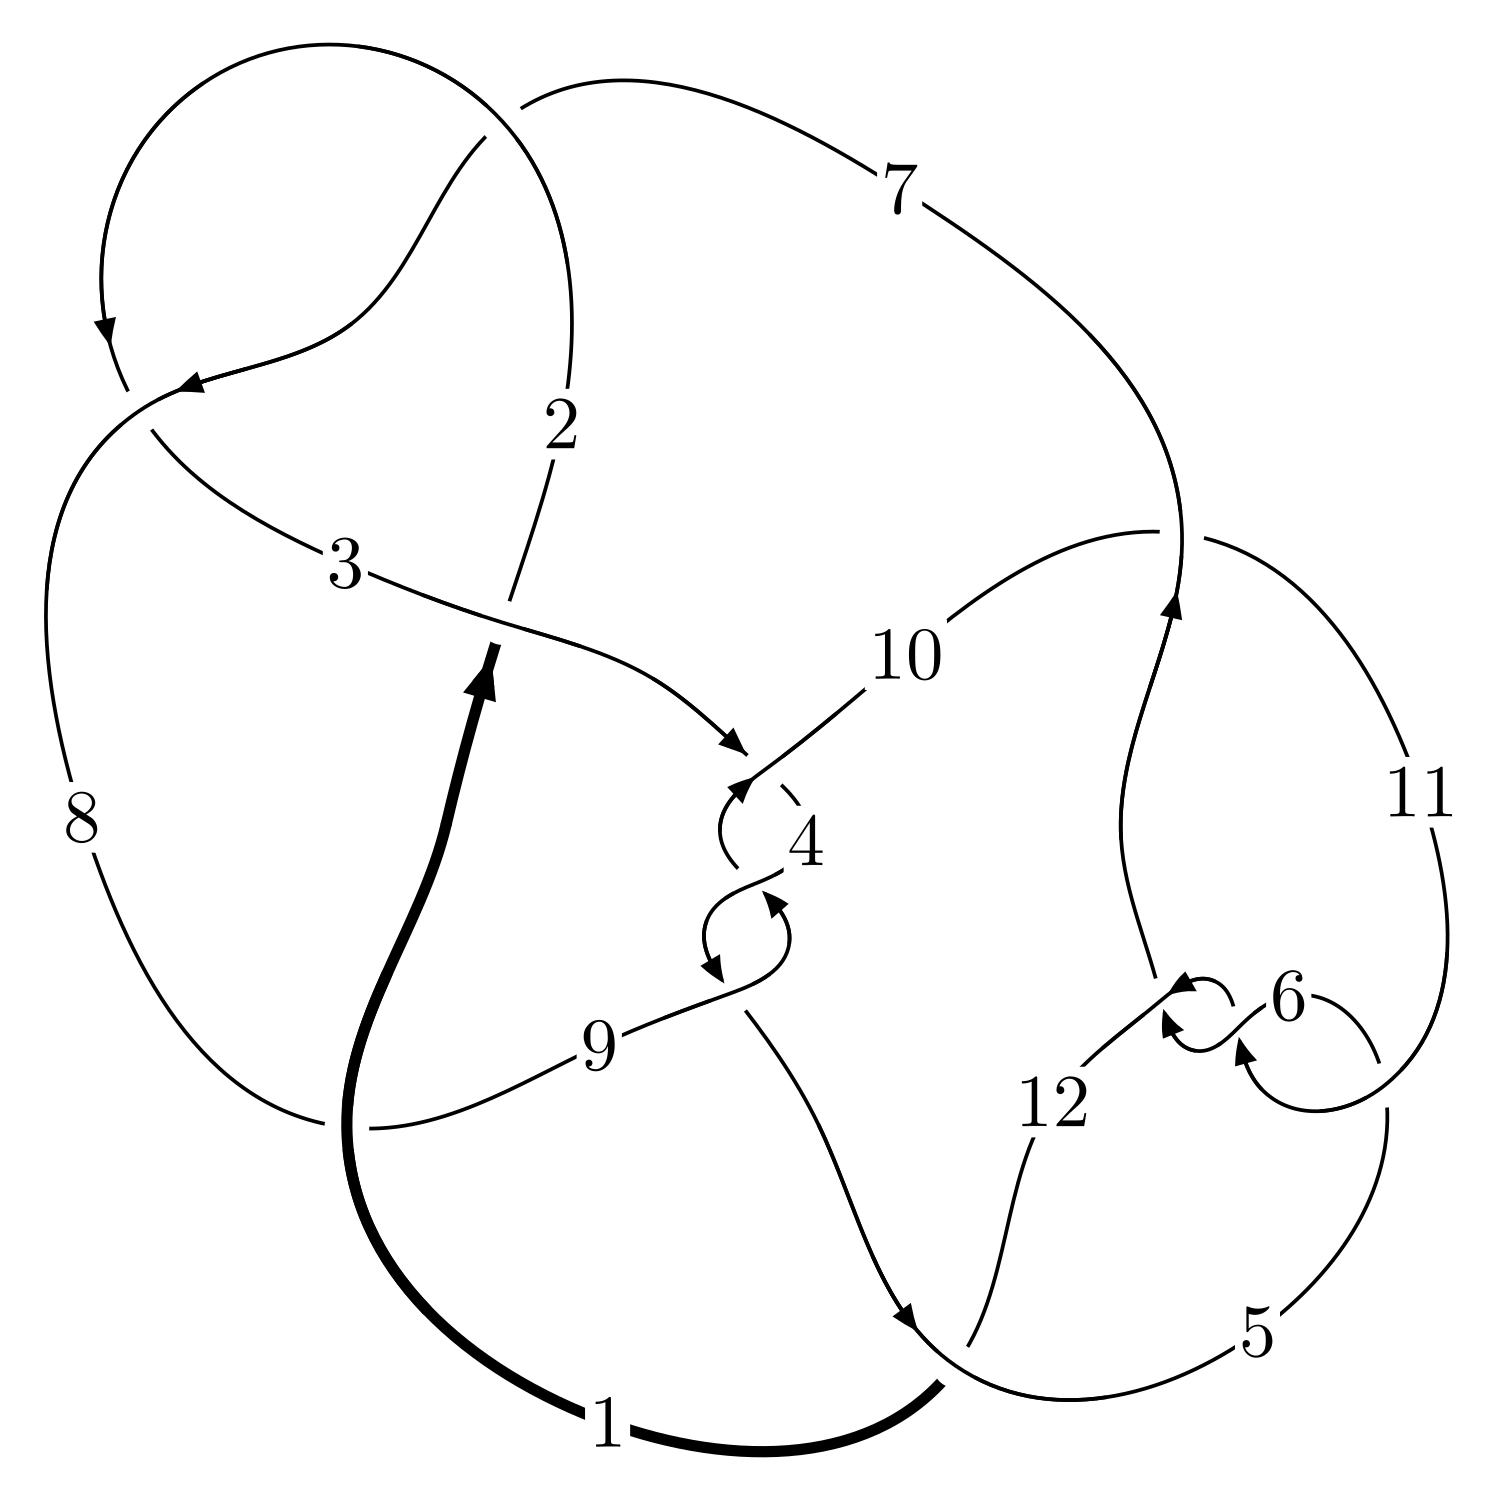
\includegraphics[width=112pt]{../../../GIT/diagram.site/Diagrams/png/1550_12a_0749.png}\\
\ \ \ A knot diagram\footnotemark}&
\allowdisplaybreaks
\textbf{Linearized knot diagam} \\
\cline{2-2}
 &
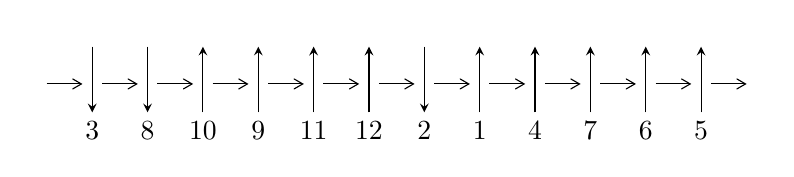
\begin{tikzpicture}[x=20pt, y=17pt]
	% nodes
	\node (C0) at (0, 0) {};
	\node (C1) at (1, 0) {};
	\node (C1U) at (1, +1) {};
	\node (C1D) at (1, -1) {3};

	\node (C2) at (2, 0) {};
	\node (C2U) at (2, +1) {};
	\node (C2D) at (2, -1) {8};

	\node (C3) at (3, 0) {};
	\node (C3U) at (3, +1) {};
	\node (C3D) at (3, -1) {10};

	\node (C4) at (4, 0) {};
	\node (C4U) at (4, +1) {};
	\node (C4D) at (4, -1) {9};

	\node (C5) at (5, 0) {};
	\node (C5U) at (5, +1) {};
	\node (C5D) at (5, -1) {11};

	\node (C6) at (6, 0) {};
	\node (C6U) at (6, +1) {};
	\node (C6D) at (6, -1) {12};

	\node (C7) at (7, 0) {};
	\node (C7U) at (7, +1) {};
	\node (C7D) at (7, -1) {2};

	\node (C8) at (8, 0) {};
	\node (C8U) at (8, +1) {};
	\node (C8D) at (8, -1) {1};

	\node (C9) at (9, 0) {};
	\node (C9U) at (9, +1) {};
	\node (C9D) at (9, -1) {4};

	\node (C10) at (10, 0) {};
	\node (C10U) at (10, +1) {};
	\node (C10D) at (10, -1) {7};

	\node (C11) at (11, 0) {};
	\node (C11U) at (11, +1) {};
	\node (C11D) at (11, -1) {6};

	\node (C12) at (12, 0) {};
	\node (C12U) at (12, +1) {};
	\node (C12D) at (12, -1) {5};
	\node (C13) at (13, 0) {};

	% arrows
	\draw[->,>={angle 60}]
	(C0) edge (C1) (C1) edge (C2) (C2) edge (C3) (C3) edge (C4) (C4) edge (C5) (C5) edge (C6) (C6) edge (C7) (C7) edge (C8) (C8) edge (C9) (C9) edge (C10) (C10) edge (C11) (C11) edge (C12) (C12) edge (C13) ;	\draw[->,>=stealth]
	(C1U) edge (C1D) (C2U) edge (C2D) (C3D) edge (C3U) (C4D) edge (C4U) (C5D) edge (C5U) (C6D) edge (C6U) (C7U) edge (C7D) (C8D) edge (C8U) (C9D) edge (C9U) (C10D) edge (C10U) (C11D) edge (C11U) (C12D) edge (C12U) ;
	\end{tikzpicture} \\
\hhline{~~} \\& 
\textbf{Solving Sequence} \\ \cline{2-2} 
 &
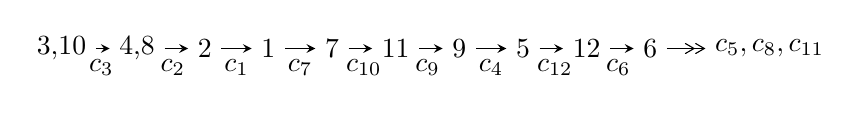
\begin{tikzpicture}[x=23pt, y=7pt]
	% node
	\node (A0) at (-1/8, 0) {3,10};
	\node (A1) at (17/16, 0) {4,8};
	\node (A2) at (17/8, 0) {2};
	\node (A3) at (25/8, 0) {1};
	\node (A4) at (33/8, 0) {7};
	\node (A5) at (41/8, 0) {11};
	\node (A6) at (49/8, 0) {9};
	\node (A7) at (57/8, 0) {5};
	\node (A8) at (65/8, 0) {12};
	\node (A9) at (73/8, 0) {6};
	\node (C1) at (1/2, -1) {$c_{3}$};
	\node (C2) at (13/8, -1) {$c_{2}$};
	\node (C3) at (21/8, -1) {$c_{1}$};
	\node (C4) at (29/8, -1) {$c_{7}$};
	\node (C5) at (37/8, -1) {$c_{10}$};
	\node (C6) at (45/8, -1) {$c_{9}$};
	\node (C7) at (53/8, -1) {$c_{4}$};
	\node (C8) at (61/8, -1) {$c_{12}$};
	\node (C9) at (69/8, -1) {$c_{6}$};
	\node (A10) at (11, 0) {$c_{5},c_{8},c_{11}$};

	% edge
	\draw[->,>=stealth]	
	(A0) edge (A1) (A1) edge (A2) (A2) edge (A3) (A3) edge (A4) (A4) edge (A5) (A5) edge (A6) (A6) edge (A7) (A7) edge (A8) (A8) edge (A9) ;
	\draw[->>,>={angle 60}]	
	(A9) edge (A10);
\end{tikzpicture} \\ 

\end{tabular} \\

\footnotetext{
The image of knot diagram is generated by the software ``\textbf{Draw programme}" developed by Andrew Bartholomew(\url{http://www.layer8.co.uk/maths/draw/index.htm\#Running-draw}), where we modified some parts for our purpose(\url{https://github.com/CATsTAILs/LinksPainter}).
}\phantom \\ \newline 
\centering \textbf{Ideals for irreducible components\footnotemark of $X_{\text{par}}$} 
 
\begin{align*}
I^u_{1}&=\langle 
1.15464\times10^{129} u^{82}-2.12036\times10^{129} u^{81}+\cdots+1.05249\times10^{130} b-2.56113\times10^{129},\\
\phantom{I^u_{1}}&\phantom{= \langle  }-2.50662\times10^{130} u^{82}+2.53263\times10^{130} u^{81}+\cdots+1.05249\times10^{130} a+1.83078\times10^{131},\\
\phantom{I^u_{1}}&\phantom{= \langle  }u^{83}- u^{82}+\cdots-16 u+1\rangle \\
I^u_{2}&=\langle 
a^4 u- a^3 u-4 a^3-5 a^2 u+3 a^2+2 a u+b+2 a,\\
\phantom{I^u_{2}}&\phantom{= \langle  }a^6+6 a^5 u- a^5-5 a^4 u-14 a^4-16 a^3 u+8 a^3+4 a^2 u+10 a^2+4 a u+a+u,\;u^2+1\rangle \\
\\
\end{align*}
\raggedright * 2 irreducible components of $\dim_{\mathbb{C}}=0$, with total 95 representations.\\
\footnotetext{All coefficients of polynomials are rational numbers. But the coefficients are sometimes approximated in decimal forms when there is not enough margin.}
\newpage
\renewcommand{\arraystretch}{1}
\centering \section*{I. $I^u_{1}= \langle 1.15\times10^{129} u^{82}-2.12\times10^{129} u^{81}+\cdots+1.05\times10^{130} b-2.56\times10^{129},\;-2.51\times10^{130} u^{82}+2.53\times10^{130} u^{81}+\cdots+1.05\times10^{130} a+1.83\times10^{131},\;u^{83}- u^{82}+\cdots-16 u+1 \rangle$}
\flushleft \textbf{(i) Arc colorings}\\
\begin{tabular}{m{7pt} m{180pt} m{7pt} m{180pt} }
\flushright $a_{3}=$&$\begin{pmatrix}1\\0\end{pmatrix}$ \\
\flushright $a_{10}=$&$\begin{pmatrix}0\\u\end{pmatrix}$ \\
\flushright $a_{4}=$&$\begin{pmatrix}1\\- u^2\end{pmatrix}$ \\
\flushright $a_{8}=$&$\begin{pmatrix}2.38162 u^{82}-2.40633 u^{81}+\cdots+211.444 u-17.3948\\-0.109706 u^{82}+0.201462 u^{81}+\cdots-12.5813 u+0.243341\end{pmatrix}$ \\
\flushright $a_{2}=$&$\begin{pmatrix}2.02156 u^{82}-1.83927 u^{81}+\cdots+180.154 u-20.2709\\-0.412232 u^{82}+0.394094 u^{81}+\cdots-14.9721 u+0.905614\end{pmatrix}$ \\
\flushright $a_{1}=$&$\begin{pmatrix}1.60933 u^{82}-1.44517 u^{81}+\cdots+165.182 u-19.3652\\-0.412232 u^{82}+0.394094 u^{81}+\cdots-14.9721 u+0.905614\end{pmatrix}$ \\
\flushright $a_{7}=$&$\begin{pmatrix}0.793212 u^{82}-0.884660 u^{81}+\cdots+82.5878 u+3.62677\\-0.0517555 u^{82}+0.217321 u^{81}+\cdots+5.93966 u-1.53522\end{pmatrix}$ \\
\flushright $a_{11}=$&$\begin{pmatrix}2.60524 u^{82}-2.10688 u^{81}+\cdots+230.248 u-16.5091\\-0.204129 u^{82}+0.0772507 u^{81}+\cdots-9.17332 u-0.257104\end{pmatrix}$ \\
\flushright $a_{9}=$&$\begin{pmatrix}- u\\u^3+u\end{pmatrix}$ \\
\flushright $a_{5}=$&$\begin{pmatrix}u^2+1\\- u^4-2 u^2\end{pmatrix}$ \\
\flushright $a_{12}=$&$\begin{pmatrix}2.04028 u^{82}-1.82475 u^{81}+\cdots+181.225 u-20.1356\\-0.453441 u^{82}+0.484379 u^{81}+\cdots-15.0883 u+0.934102\end{pmatrix}$ \\
\flushright $a_{6}=$&$\begin{pmatrix}3.21049 u^{82}-3.23128 u^{81}+\cdots+320.180 u-24.9601\\0.0333591 u^{82}+0.0548937 u^{81}+\cdots-18.6788 u+0.279037\end{pmatrix}$\\&\end{tabular}
\flushleft \textbf{(ii) Obstruction class $= -1$}\\~\\
\flushleft \textbf{(iii) Cusp Shapes $= 0.292915 u^{82}-0.00299820 u^{81}+\cdots-0.231972 u+11.2199$}\\~\\
\newpage\renewcommand{\arraystretch}{1}
\flushleft \textbf{(iv) u-Polynomials at the component}\newline \\
\begin{tabular}{m{50pt}|m{274pt}}
Crossings & \hspace{64pt}u-Polynomials at each crossing \\
\hline $$\begin{aligned}c_{1}\end{aligned}$$&$\begin{aligned}
&u^{83}+43 u^{82}+\cdots+210 u+25
\end{aligned}$\\
\hline $$\begin{aligned}c_{2},c_{7}\end{aligned}$$&$\begin{aligned}
&u^{83}+u^{82}+\cdots+21 u^2-5
\end{aligned}$\\
\hline $$\begin{aligned}c_{3},c_{4},c_{9}\end{aligned}$$&$\begin{aligned}
&u^{83}+u^{82}+\cdots-16 u-1
\end{aligned}$\\
\hline $$\begin{aligned}c_{5},c_{6},c_{11}\end{aligned}$$&$\begin{aligned}
&u^{83}+u^{82}+\cdots-10 u-1
\end{aligned}$\\
\hline $$\begin{aligned}c_{8}\end{aligned}$$&$\begin{aligned}
&u^{83}+3 u^{82}+\cdots+21790 u-3655
\end{aligned}$\\
\hline $$\begin{aligned}c_{10},c_{12}\end{aligned}$$&$\begin{aligned}
&u^{83}-3 u^{82}+\cdots+4852 u+517
\end{aligned}$\\
\hline
\end{tabular}\\~\\
\newpage\renewcommand{\arraystretch}{1}
\flushleft \textbf{(v) Riley Polynomials at the component}\newline \\
\begin{tabular}{m{50pt}|m{274pt}}
Crossings & \hspace{64pt}Riley Polynomials at each crossing \\
\hline $$\begin{aligned}c_{1}\end{aligned}$$&$\begin{aligned}
&y^{83}+y^{82}+\cdots+4550 y-625
\end{aligned}$\\
\hline $$\begin{aligned}c_{2},c_{7}\end{aligned}$$&$\begin{aligned}
&y^{83}-43 y^{82}+\cdots+210 y-25
\end{aligned}$\\
\hline $$\begin{aligned}c_{3},c_{4},c_{9}\end{aligned}$$&$\begin{aligned}
&y^{83}+83 y^{82}+\cdots+88 y-1
\end{aligned}$\\
\hline $$\begin{aligned}c_{5},c_{6},c_{11}\end{aligned}$$&$\begin{aligned}
&y^{83}-69 y^{82}+\cdots+44 y-1
\end{aligned}$\\
\hline $$\begin{aligned}c_{8}\end{aligned}$$&$\begin{aligned}
&y^{83}+41 y^{82}+\cdots+762679210 y-13359025
\end{aligned}$\\
\hline $$\begin{aligned}c_{10},c_{12}\end{aligned}$$&$\begin{aligned}
&y^{83}+63 y^{82}+\cdots+14835624 y-267289
\end{aligned}$\\
\hline
\end{tabular}\\~\\
\newpage\flushleft \textbf{(vi) Complex Volumes and Cusp Shapes}
$$\begin{array}{c|c|c}  
\text{Solutions to }I^u_{1}& \I (\text{vol} + \sqrt{-1}CS) & \text{Cusp shape}\\
 \hline 
\begin{aligned}
u &= \phantom{-}0.828176 + 0.557418 I \\
a &= \phantom{-}0.26185 - 1.69427 I \\
b &= -1.155510 + 0.462789 I\end{aligned}
 & -2.43646 + 2.58116 I & \phantom{-0.000000 } 0 \\ \hline\begin{aligned}
u &= \phantom{-}0.828176 - 0.557418 I \\
a &= \phantom{-}0.26185 + 1.69427 I \\
b &= -1.155510 - 0.462789 I\end{aligned}
 & -2.43646 - 2.58116 I & \phantom{-0.000000 } 0 \\ \hline\begin{aligned}
u &= -0.880668 + 0.478159 I \\
a &= -0.35382 - 1.77762 I \\
b &= \phantom{-}1.159560 + 0.498988 I\end{aligned}
 & -5.82520 - 6.87062 I & \phantom{-0.000000 } 0 \\ \hline\begin{aligned}
u &= -0.880668 - 0.478159 I \\
a &= -0.35382 + 1.77762 I \\
b &= \phantom{-}1.159560 - 0.498988 I\end{aligned}
 & -5.82520 + 6.87062 I & \phantom{-0.000000 } 0 \\ \hline\begin{aligned}
u &= \phantom{-}0.913983 + 0.416889 I \\
a &= \phantom{-}0.42302 - 1.83644 I \\
b &= -1.159300 + 0.525076 I\end{aligned}
 & -1.42155 + 11.14220 I & \phantom{-0.000000 } 0 \\ \hline\begin{aligned}
u &= \phantom{-}0.913983 - 0.416889 I \\
a &= \phantom{-}0.42302 + 1.83644 I \\
b &= -1.159300 - 0.525076 I\end{aligned}
 & -1.42155 - 11.14220 I & \phantom{-0.000000 } 0 \\ \hline\begin{aligned}
u &= \phantom{-}0.792210 + 0.634260 I \\
a &= -0.556105 - 0.320556 I \\
b &= \phantom{-}1.160410 + 0.345717 I\end{aligned}
 & -2.67272 + 2.90389 I & \phantom{-0.000000 } 0 \\ \hline\begin{aligned}
u &= \phantom{-}0.792210 - 0.634260 I \\
a &= -0.556105 + 0.320556 I \\
b &= \phantom{-}1.160410 - 0.345717 I\end{aligned}
 & -2.67272 - 2.90389 I & \phantom{-0.000000 } 0 \\ \hline\begin{aligned}
u &= -0.084056 + 1.041490 I \\
a &= \phantom{-}0.000756 - 1.089570 I \\
b &= \phantom{-}0.800253 + 0.494787 I\end{aligned}
 & -1.54448 - 2.06060 I & \phantom{-0.000000 } 0 \\ \hline\begin{aligned}
u &= -0.084056 - 1.041490 I \\
a &= \phantom{-}0.000756 + 1.089570 I \\
b &= \phantom{-}0.800253 - 0.494787 I\end{aligned}
 & -1.54448 + 2.06060 I & \phantom{-0.000000 } 0\\
 \hline 
 \end{array}$$\newpage$$\begin{array}{c|c|c}  
\text{Solutions to }I^u_{1}& \I (\text{vol} + \sqrt{-1}CS) & \text{Cusp shape}\\
 \hline 
\begin{aligned}
u &= -0.754065 + 0.726286 I \\
a &= \phantom{-}0.524056 - 0.394935 I \\
b &= -1.155730 + 0.389682 I\end{aligned}
 & -6.60258 + 1.33321 I & \phantom{-0.000000 } 0 \\ \hline\begin{aligned}
u &= -0.754065 - 0.726286 I \\
a &= \phantom{-}0.524056 + 0.394935 I \\
b &= -1.155730 - 0.389682 I\end{aligned}
 & -6.60258 - 1.33321 I & \phantom{-0.000000 } 0 \\ \hline\begin{aligned}
u &= -0.378493 + 1.015650 I \\
a &= \phantom{-}0.165756 - 1.219100 I \\
b &= \phantom{-}0.970336 + 0.171230 I\end{aligned}
 & -0.90265 - 3.43454 I & \phantom{-0.000000 } 0 \\ \hline\begin{aligned}
u &= -0.378493 - 1.015650 I \\
a &= \phantom{-}0.165756 + 1.219100 I \\
b &= \phantom{-}0.970336 - 0.171230 I\end{aligned}
 & -0.90265 + 3.43454 I & \phantom{-0.000000 } 0 \\ \hline\begin{aligned}
u &= \phantom{-}0.720759 + 0.819102 I \\
a &= -0.503846 - 0.474505 I \\
b &= \phantom{-}1.152480 + 0.431957 I\end{aligned}
 & -2.66068 - 5.56325 I & \phantom{-0.000000 } 0 \\ \hline\begin{aligned}
u &= \phantom{-}0.720759 - 0.819102 I \\
a &= -0.503846 + 0.474505 I \\
b &= \phantom{-}1.152480 - 0.431957 I\end{aligned}
 & -2.66068 + 5.56325 I & \phantom{-0.000000 } 0 \\ \hline\begin{aligned}
u &= \phantom{-}0.255809 + 1.067630 I \\
a &= -0.155725 - 1.352350 I \\
b &= -0.795173 + 0.055550 I\end{aligned}
 & -3.85075 + 0.27233 I & \phantom{-0.000000 } 0 \\ \hline\begin{aligned}
u &= \phantom{-}0.255809 - 1.067630 I \\
a &= -0.155725 + 1.352350 I \\
b &= -0.795173 - 0.055550 I\end{aligned}
 & -3.85075 - 0.27233 I & \phantom{-0.000000 } 0 \\ \hline\begin{aligned}
u &= -0.204373 + 1.083280 I \\
a &= -0.01086 - 1.54055 I \\
b &= \phantom{-}0.683616 - 0.078181 I\end{aligned}
 & \phantom{-}0.80097 + 3.01593 I & \phantom{-0.000000 } 0 \\ \hline\begin{aligned}
u &= -0.204373 - 1.083280 I \\
a &= -0.01086 + 1.54055 I \\
b &= \phantom{-}0.683616 + 0.078181 I\end{aligned}
 & \phantom{-}0.80097 - 3.01593 I & \phantom{-0.000000 } 0\\
 \hline 
 \end{array}$$\newpage$$\begin{array}{c|c|c}  
\text{Solutions to }I^u_{1}& \I (\text{vol} + \sqrt{-1}CS) & \text{Cusp shape}\\
 \hline 
\begin{aligned}
u &= -0.782147 + 0.421744 I \\
a &= \phantom{-}0.65089 - 1.35866 I \\
b &= -0.212910 + 0.749136 I\end{aligned}
 & \phantom{-}1.33540 - 6.35685 I & \phantom{-}6.00000 + 5.58288 I \\ \hline\begin{aligned}
u &= -0.782147 - 0.421744 I \\
a &= \phantom{-}0.65089 + 1.35866 I \\
b &= -0.212910 - 0.749136 I\end{aligned}
 & \phantom{-}1.33540 + 6.35685 I & \phantom{-}6.00000 - 5.58288 I \\ \hline\begin{aligned}
u &= -0.621544 + 0.602167 I \\
a &= \phantom{-}0.432472 - 1.247140 I \\
b &= -0.056022 + 0.667459 I\end{aligned}
 & \phantom{-}0.62596 + 1.63981 I & \phantom{-}6.00000 + 0. I\phantom{ +0.000000I} \\ \hline\begin{aligned}
u &= -0.621544 - 0.602167 I \\
a &= \phantom{-}0.432472 + 1.247140 I \\
b &= -0.056022 - 0.667459 I\end{aligned}
 & \phantom{-}0.62596 - 1.63981 I & \phantom{-}6.00000 + 0. I\phantom{ +0.000000I} \\ \hline\begin{aligned}
u &= \phantom{-}0.710823 + 0.487393 I \\
a &= -0.57026 - 1.29476 I \\
b &= \phantom{-}0.155215 + 0.709269 I\end{aligned}
 & -2.94696 + 2.31361 I & \phantom{-}3.43042 - 3.33064 I \\ \hline\begin{aligned}
u &= \phantom{-}0.710823 - 0.487393 I \\
a &= -0.57026 + 1.29476 I \\
b &= \phantom{-}0.155215 - 0.709269 I\end{aligned}
 & -2.94696 - 2.31361 I & \phantom{-}3.43042 + 3.33064 I \\ \hline\begin{aligned}
u &= -0.287984 + 1.116130 I \\
a &= \phantom{-}0.259716 - 0.868717 I \\
b &= -0.993147 + 0.583252 I\end{aligned}
 & \phantom{-}1.74339 + 2.15963 I & \phantom{-0.000000 } 0 \\ \hline\begin{aligned}
u &= -0.287984 - 1.116130 I \\
a &= \phantom{-}0.259716 + 0.868717 I \\
b &= -0.993147 - 0.583252 I\end{aligned}
 & \phantom{-}1.74339 - 2.15963 I & \phantom{-0.000000 } 0 \\ \hline\begin{aligned}
u &= \phantom{-}0.279482 + 1.139960 I \\
a &= \phantom{-}0.020964 - 1.246390 I \\
b &= -0.565039 + 0.608087 I\end{aligned}
 & \phantom{-}2.98511 + 2.56133 I & \phantom{-0.000000 } 0 \\ \hline\begin{aligned}
u &= \phantom{-}0.279482 - 1.139960 I \\
a &= \phantom{-}0.020964 + 1.246390 I \\
b &= -0.565039 - 0.608087 I\end{aligned}
 & \phantom{-}2.98511 - 2.56133 I & \phantom{-0.000000 } 0\\
 \hline 
 \end{array}$$\newpage$$\begin{array}{c|c|c}  
\text{Solutions to }I^u_{1}& \I (\text{vol} + \sqrt{-1}CS) & \text{Cusp shape}\\
 \hline 
\begin{aligned}
u &= \phantom{-}0.176144 + 1.296320 I \\
a &= \phantom{-}0.611233 - 0.029819 I \\
b &= -0.248951 - 0.649703 I\end{aligned}
 & \phantom{-}1.94452 + 3.81460 I & \phantom{-0.000000 } 0 \\ \hline\begin{aligned}
u &= \phantom{-}0.176144 - 1.296320 I \\
a &= \phantom{-}0.611233 + 0.029819 I \\
b &= -0.248951 + 0.649703 I\end{aligned}
 & \phantom{-}1.94452 - 3.81460 I & \phantom{-0.000000 } 0 \\ \hline\begin{aligned}
u &= \phantom{-}0.649068 + 0.077548 I \\
a &= -1.19948 - 1.21441 I \\
b &= \phantom{-}0.465751 + 0.631327 I\end{aligned}
 & \phantom{-}6.17107 + 0.86345 I & \phantom{-}14.3969 - 0.7384 I \\ \hline\begin{aligned}
u &= \phantom{-}0.649068 - 0.077548 I \\
a &= -1.19948 + 1.21441 I \\
b &= \phantom{-}0.465751 - 0.631327 I\end{aligned}
 & \phantom{-}6.17107 - 0.86345 I & \phantom{-}14.3969 + 0.7384 I \\ \hline\begin{aligned}
u &= -0.610090 + 0.179998 I \\
a &= -0.14723 - 2.51696 I \\
b &= \phantom{-}1.030630 + 0.544608 I\end{aligned}
 & \phantom{-}4.53717 - 5.47882 I & \phantom{-}11.04158 + 6.52708 I \\ \hline\begin{aligned}
u &= -0.610090 - 0.179998 I \\
a &= -0.14723 + 2.51696 I \\
b &= \phantom{-}1.030630 - 0.544608 I\end{aligned}
 & \phantom{-}4.53717 + 5.47882 I & \phantom{-}11.04158 - 6.52708 I \\ \hline\begin{aligned}
u &= \phantom{-}0.477840 + 0.410372 I \\
a &= -0.36614 - 1.97770 I \\
b &= -1.023630 + 0.465904 I\end{aligned}
 & -0.86580 + 4.07227 I & \phantom{-}5.56865 - 9.23249 I \\ \hline\begin{aligned}
u &= \phantom{-}0.477840 - 0.410372 I \\
a &= -0.36614 + 1.97770 I \\
b &= -1.023630 - 0.465904 I\end{aligned}
 & -0.86580 - 4.07227 I & \phantom{-}5.56865 + 9.23249 I \\ \hline\begin{aligned}
u &= -0.067862 + 1.384400 I \\
a &= -0.196273 + 0.154900 I \\
b &= \phantom{-}0.083261 - 0.720975 I\end{aligned}
 & -3.97118 - 1.82061 I & \phantom{-0.000000 } 0 \\ \hline\begin{aligned}
u &= -0.067862 - 1.384400 I \\
a &= -0.196273 - 0.154900 I \\
b &= \phantom{-}0.083261 + 0.720975 I\end{aligned}
 & -3.97118 + 1.82061 I & \phantom{-0.000000 } 0\\
 \hline 
 \end{array}$$\newpage$$\begin{array}{c|c|c}  
\text{Solutions to }I^u_{1}& \I (\text{vol} + \sqrt{-1}CS) & \text{Cusp shape}\\
 \hline 
\begin{aligned}
u &= \phantom{-}0.001191 + 1.386730 I \\
a &= \phantom{-}1.57028 + 0.32567 I \\
b &= \phantom{-}1.114940 - 0.388135 I\end{aligned}
 & -1.50250 - 0.63171 I & \phantom{-0.000000 } 0 \\ \hline\begin{aligned}
u &= \phantom{-}0.001191 - 1.386730 I \\
a &= \phantom{-}1.57028 - 0.32567 I \\
b &= \phantom{-}1.114940 + 0.388135 I\end{aligned}
 & -1.50250 + 0.63171 I & \phantom{-0.000000 } 0 \\ \hline\begin{aligned}
u &= \phantom{-}0.028734 + 1.407100 I \\
a &= -0.278899 - 1.167510 I \\
b &= \phantom{-}0.869859 + 0.754641 I\end{aligned}
 & -1.95541 + 1.26508 I & \phantom{-0.000000 } 0 \\ \hline\begin{aligned}
u &= \phantom{-}0.028734 - 1.407100 I \\
a &= -0.278899 + 1.167510 I \\
b &= \phantom{-}0.869859 - 0.754641 I\end{aligned}
 & -1.95541 - 1.26508 I & \phantom{-0.000000 } 0 \\ \hline\begin{aligned}
u &= \phantom{-}0.045458 + 1.407770 I \\
a &= \phantom{-}0.248108 - 1.206250 I \\
b &= -0.824993 + 0.766512 I\end{aligned}
 & -5.76997 + 2.85289 I & \phantom{-0.000000 } 0 \\ \hline\begin{aligned}
u &= \phantom{-}0.045458 - 1.407770 I \\
a &= \phantom{-}0.248108 + 1.206250 I \\
b &= -0.824993 - 0.766512 I\end{aligned}
 & -5.76997 - 2.85289 I & \phantom{-0.000000 } 0 \\ \hline\begin{aligned}
u &= -0.586055\phantom{ +0.000000I} \\
a &= \phantom{-}0.708998\phantom{ +0.000000I} \\
b &= -0.913508\phantom{ +0.000000I}\end{aligned}
 & \phantom{-}1.91063\phantom{ +0.000000I} & \phantom{-}6.04100\phantom{ +0.000000I} \\ \hline\begin{aligned}
u &= -0.11242 + 1.41303 I \\
a &= -0.224623 - 1.243150 I \\
b &= \phantom{-}0.783760 + 0.782633 I\end{aligned}
 & -1.69873 - 6.98576 I & \phantom{-0.000000 } 0 \\ \hline\begin{aligned}
u &= -0.11242 - 1.41303 I \\
a &= -0.224623 + 1.243150 I \\
b &= \phantom{-}0.783760 - 0.782633 I\end{aligned}
 & -1.69873 + 6.98576 I & \phantom{-0.000000 } 0 \\ \hline\begin{aligned}
u &= -0.20015 + 1.40506 I \\
a &= -1.30473 + 1.45890 I \\
b &= -1.132050 - 0.511264 I\end{aligned}
 & -0.59248 - 8.34419 I & \phantom{-0.000000 } 0\\
 \hline 
 \end{array}$$\newpage$$\begin{array}{c|c|c}  
\text{Solutions to }I^u_{1}& \I (\text{vol} + \sqrt{-1}CS) & \text{Cusp shape}\\
 \hline 
\begin{aligned}
u &= -0.20015 - 1.40506 I \\
a &= -1.30473 - 1.45890 I \\
b &= -1.132050 + 0.511264 I\end{aligned}
 & -0.59248 + 8.34419 I & \phantom{-0.000000 } 0 \\ \hline\begin{aligned}
u &= -0.04676 + 1.47166 I \\
a &= -1.166650 + 0.648335 I \\
b &= -1.170280 - 0.419278 I\end{aligned}
 & -7.49627 - 2.14085 I & \phantom{-0.000000 } 0 \\ \hline\begin{aligned}
u &= -0.04676 - 1.47166 I \\
a &= -1.166650 - 0.648335 I \\
b &= -1.170280 + 0.419278 I\end{aligned}
 & -7.49627 + 2.14085 I & \phantom{-0.000000 } 0 \\ \hline\begin{aligned}
u &= \phantom{-}0.13948 + 1.47980 I \\
a &= \phantom{-}1.09205 + 1.05374 I \\
b &= \phantom{-}1.173810 - 0.475339 I\end{aligned}
 & -7.09658 + 6.25907 I & \phantom{-0.000000 } 0 \\ \hline\begin{aligned}
u &= \phantom{-}0.13948 - 1.47980 I \\
a &= \phantom{-}1.09205 - 1.05374 I \\
b &= \phantom{-}1.173810 + 0.475339 I\end{aligned}
 & -7.09658 - 6.25907 I & \phantom{-0.000000 } 0 \\ \hline\begin{aligned}
u &= -0.29281 + 1.49818 I \\
a &= -0.618256 + 0.621581 I \\
b &= \phantom{-}0.275741 - 0.898548 I\end{aligned}
 & -4.88602 - 10.29530 I & \phantom{-0.000000 } 0 \\ \hline\begin{aligned}
u &= -0.29281 - 1.49818 I \\
a &= -0.618256 - 0.621581 I \\
b &= \phantom{-}0.275741 + 0.898548 I\end{aligned}
 & -4.88602 + 10.29530 I & \phantom{-0.000000 } 0 \\ \hline\begin{aligned}
u &= -0.444092 + 0.145528 I \\
a &= \phantom{-}0.978477 - 0.640428 I \\
b &= -0.408435 + 0.412605 I\end{aligned}
 & \phantom{-}0.852672 - 0.232931 I & \phantom{-}12.03073 + 2.51602 I \\ \hline\begin{aligned}
u &= -0.444092 - 0.145528 I \\
a &= \phantom{-}0.978477 + 0.640428 I \\
b &= -0.408435 - 0.412605 I\end{aligned}
 & \phantom{-}0.852672 + 0.232931 I & \phantom{-}12.03073 - 2.51602 I \\ \hline\begin{aligned}
u &= -0.20380 + 1.52010 I \\
a &= -0.431672 + 0.572184 I \\
b &= \phantom{-}0.193463 - 0.891300 I\end{aligned}
 & -6.27329 - 1.34438 I & \phantom{-0.000000 } 0\\
 \hline 
 \end{array}$$\newpage$$\begin{array}{c|c|c}  
\text{Solutions to }I^u_{1}& \I (\text{vol} + \sqrt{-1}CS) & \text{Cusp shape}\\
 \hline 
\begin{aligned}
u &= -0.20380 - 1.52010 I \\
a &= -0.431672 - 0.572184 I \\
b &= \phantom{-}0.193463 + 0.891300 I\end{aligned}
 & -6.27329 + 1.34438 I & \phantom{-0.000000 } 0 \\ \hline\begin{aligned}
u &= \phantom{-}0.25612 + 1.51278 I \\
a &= \phantom{-}0.537026 + 0.607048 I \\
b &= -0.240717 - 0.899184 I\end{aligned}
 & -9.45956 + 5.87960 I & \phantom{-0.000000 } 0 \\ \hline\begin{aligned}
u &= \phantom{-}0.25612 - 1.51278 I \\
a &= \phantom{-}0.537026 - 0.607048 I \\
b &= -0.240717 + 0.899184 I\end{aligned}
 & -9.45956 - 5.87960 I & \phantom{-0.000000 } 0 \\ \hline\begin{aligned}
u &= \phantom{-}0.34667 + 1.51698 I \\
a &= \phantom{-}0.59504 + 1.62681 I \\
b &= \phantom{-}1.193840 - 0.587206 I\end{aligned}
 & -7.6640 + 15.7308 I & \phantom{-0.000000 } 0 \\ \hline\begin{aligned}
u &= \phantom{-}0.34667 - 1.51698 I \\
a &= \phantom{-}0.59504 - 1.62681 I \\
b &= \phantom{-}1.193840 + 0.587206 I\end{aligned}
 & -7.6640 - 15.7308 I & \phantom{-0.000000 } 0 \\ \hline\begin{aligned}
u &= \phantom{-}0.023429 + 0.440080 I \\
a &= \phantom{-}0.993538 - 0.407074 I \\
b &= \phantom{-}0.936093 + 0.425987 I\end{aligned}
 & -1.28387 - 1.68323 I & \phantom{-}3.77150 - 0.35257 I \\ \hline\begin{aligned}
u &= \phantom{-}0.023429 - 0.440080 I \\
a &= \phantom{-}0.993538 + 0.407074 I \\
b &= \phantom{-}0.936093 - 0.425987 I\end{aligned}
 & -1.28387 + 1.68323 I & \phantom{-}3.77150 + 0.35257 I \\ \hline\begin{aligned}
u &= -0.399913 + 0.171939 I \\
a &= \phantom{-}2.65180 + 1.24043 I \\
b &= -0.711891 - 0.566818 I\end{aligned}
 & \phantom{-}3.50631 - 5.22844 I & \phantom{-}11.78714 + 6.73129 I \\ \hline\begin{aligned}
u &= -0.399913 - 0.171939 I \\
a &= \phantom{-}2.65180 - 1.24043 I \\
b &= -0.711891 + 0.566818 I\end{aligned}
 & \phantom{-}3.50631 + 5.22844 I & \phantom{-}11.78714 - 6.73129 I \\ \hline\begin{aligned}
u &= -0.31801 + 1.53692 I \\
a &= -0.61042 + 1.52370 I \\
b &= -1.204090 - 0.572653 I\end{aligned}
 & -12.3754 - 11.2511 I & \phantom{-0.000000 } 0\\
 \hline 
 \end{array}$$\newpage$$\begin{array}{c|c|c}  
\text{Solutions to }I^u_{1}& \I (\text{vol} + \sqrt{-1}CS) & \text{Cusp shape}\\
 \hline 
\begin{aligned}
u &= -0.31801 - 1.53692 I \\
a &= -0.61042 - 1.52370 I \\
b &= -1.204090 + 0.572653 I\end{aligned}
 & -12.3754 + 11.2511 I & \phantom{-0.000000 } 0 \\ \hline\begin{aligned}
u &= \phantom{-}0.27270 + 1.55039 I \\
a &= \phantom{-}0.66002 + 1.38973 I \\
b &= \phantom{-}1.211490 - 0.549265 I\end{aligned}
 & -9.35289 + 6.58290 I & \phantom{-0.000000 } 0 \\ \hline\begin{aligned}
u &= \phantom{-}0.27270 - 1.55039 I \\
a &= \phantom{-}0.66002 - 1.38973 I \\
b &= \phantom{-}1.211490 + 0.549265 I\end{aligned}
 & -9.35289 - 6.58290 I & \phantom{-0.000000 } 0 \\ \hline\begin{aligned}
u &= \phantom{-}0.23240 + 1.57121 I \\
a &= -0.456742 - 0.075976 I \\
b &= -1.267760 - 0.252241 I\end{aligned}
 & -9.99924 + 6.60552 I & \phantom{-0.000000 } 0 \\ \hline\begin{aligned}
u &= \phantom{-}0.23240 - 1.57121 I \\
a &= -0.456742 + 0.075976 I \\
b &= -1.267760 + 0.252241 I\end{aligned}
 & -9.99924 - 6.60552 I & \phantom{-0.000000 } 0 \\ \hline\begin{aligned}
u &= -0.18866 + 1.59001 I \\
a &= \phantom{-}0.490949 + 0.040309 I \\
b &= \phantom{-}1.270750 - 0.282944 I\end{aligned}
 & -14.4041 - 2.0103 I & \phantom{-0.000000 } 0 \\ \hline\begin{aligned}
u &= -0.18866 - 1.59001 I \\
a &= \phantom{-}0.490949 - 0.040309 I \\
b &= \phantom{-}1.270750 + 0.282944 I\end{aligned}
 & -14.4041 + 2.0103 I & \phantom{-0.000000 } 0 \\ \hline\begin{aligned}
u &= \phantom{-}0.13358 + 1.59807 I \\
a &= -0.552059 + 0.174631 I \\
b &= -1.266410 - 0.318036 I\end{aligned}
 & -10.97300 - 2.69837 I & \phantom{-0.000000 } 0 \\ \hline\begin{aligned}
u &= \phantom{-}0.13358 - 1.59807 I \\
a &= -0.552059 - 0.174631 I \\
b &= -1.266410 + 0.318036 I\end{aligned}
 & -10.97300 + 2.69837 I & \phantom{-0.000000 } 0 \\ \hline\begin{aligned}
u &= \phantom{-}0.301350 + 0.041219 I \\
a &= -2.81466 - 0.24393 I \\
b &= \phantom{-}0.742127 - 0.477090 I\end{aligned}
 & -0.90760 + 1.95680 I & \phantom{-}5.79568 - 4.89911 I\\
 \hline 
 \end{array}$$\newpage$$\begin{array}{c|c|c}  
\text{Solutions to }I^u_{1}& \I (\text{vol} + \sqrt{-1}CS) & \text{Cusp shape}\\
 \hline 
\begin{aligned}
u &= \phantom{-}0.301350 - 0.041219 I \\
a &= -2.81466 + 0.24393 I \\
b &= \phantom{-}0.742127 + 0.477090 I\end{aligned}
 & -0.90760 - 1.95680 I & \phantom{-}5.79568 + 4.89911 I \\ \hline\begin{aligned}
u &= \phantom{-}0.0855141 + 0.0580346 I \\
a &= \phantom{-}1.99596 + 11.61360 I \\
b &= -0.878605 - 0.525027 I\end{aligned}
 & \phantom{-}3.03134 + 0.82073 I & \phantom{-}11.47240 + 0.34762 I \\ \hline\begin{aligned}
u &= \phantom{-}0.0855141 - 0.0580346 I \\
a &= \phantom{-}1.99596 - 11.61360 I \\
b &= -0.878605 + 0.525027 I\end{aligned}
 & \phantom{-}3.03134 - 0.82073 I & \phantom{-}11.47240 - 0.34762 I\\
 \hline 
 \end{array}$$\newpage\newpage\renewcommand{\arraystretch}{1}
\centering \section*{II. $I^u_{2}= \langle a^4 u- a^3 u-4 a^3-5 a^2 u+3 a^2+2 a u+b+2 a,\;6 a^5 u-5 a^4 u+\cdots+10 a^2+a,\;u^2+1 \rangle$}
\flushleft \textbf{(i) Arc colorings}\\
\begin{tabular}{m{7pt} m{180pt} m{7pt} m{180pt} }
\flushright $a_{3}=$&$\begin{pmatrix}1\\0\end{pmatrix}$ \\
\flushright $a_{10}=$&$\begin{pmatrix}0\\u\end{pmatrix}$ \\
\flushright $a_{4}=$&$\begin{pmatrix}1\\1\end{pmatrix}$ \\
\flushright $a_{8}=$&$\begin{pmatrix}a\\- a^4 u+a^3 u+4 a^3+5 a^2 u-3 a^2-2 a u-2 a\end{pmatrix}$ \\
\flushright $a_{2}=$&$\begin{pmatrix}a^5 u- a^4 u-4 a^4-5 a^3 u+3 a^3+2 a^2 u+2 a^2+1\\- a^4-4 a^3 u+a^3+3 a^2 u+5 a^2+2 a u-2 a-1\end{pmatrix}$ \\
\flushright $a_{1}=$&$\begin{pmatrix}a^5 u- a^4 u-5 a^4-9 a^3 u+4 a^3+5 a^2 u+7 a^2+2 a u-2 a\\- a^4-4 a^3 u+a^3+3 a^2 u+5 a^2+2 a u-2 a-1\end{pmatrix}$ \\
\flushright $a_{7}=$&$\begin{pmatrix}- a^5-5 a^4 u+a^4+4 a^3 u+9 a^3+7 a^2 u-5 a^2-2 a u-2 a\\- a^4 u+a^3 u+4 a^3+5 a^2 u-3 a^2-2 a u-2 a- u\end{pmatrix}$ \\
\flushright $a_{11}=$&$\begin{pmatrix}- a^3 u+3 a^2+3 a u+u-1\\a+2 u\end{pmatrix}$ \\
\flushright $a_{9}=$&$\begin{pmatrix}- u\\0\end{pmatrix}$ \\
\flushright $a_{5}=$&$\begin{pmatrix}0\\1\end{pmatrix}$ \\
\flushright $a_{12}=$&$\begin{pmatrix}a^5 u- a^4 u-5 a^4-9 a^3 u+4 a^3+5 a^2 u+7 a^2+2 a u-2 a\\a^5 u- a^4 u-6 a^4-13 a^3 u+5 a^3+8 a^2 u+12 a^2+4 a u-4 a-1\end{pmatrix}$ \\
\flushright $a_{6}=$&$\begin{pmatrix}- a^5-5 a^4 u+a^4+4 a^3 u+10 a^3+10 a^2 u-5 a^2-2 a u-5 a- u\\- a^4 u+5 a^3+9 a^2 u+a u-7 a-2 u-1\end{pmatrix}$\\&\end{tabular}
\flushleft \textbf{(ii) Obstruction class $= 1$}\\~\\
\flushleft \textbf{(iii) Cusp Shapes $= -4 a^5-20 a^4 u+8 a^4+32 a^3 u+32 a^3+16 a^2 u-40 a^2-16 a u+4$}\\~\\
\newpage\renewcommand{\arraystretch}{1}
\flushleft \textbf{(iv) u-Polynomials at the component}\newline \\
\begin{tabular}{m{50pt}|m{274pt}}
Crossings & \hspace{64pt}u-Polynomials at each crossing \\
\hline $$\begin{aligned}c_{1}\end{aligned}$$&$\begin{aligned}
&(u^2- u+1)^6
\end{aligned}$\\
\hline $$\begin{aligned}c_{2},c_{7},c_{8}\end{aligned}$$&$\begin{aligned}
&(u^4- u^2+1)^3
\end{aligned}$\\
\hline $$\begin{aligned}c_{3},c_{4},c_{9}\end{aligned}$$&$\begin{aligned}
&(u^2+1)^6
\end{aligned}$\\
\hline $$\begin{aligned}c_{5},c_{6},c_{11}\end{aligned}$$&$\begin{aligned}
&(u^6-3 u^4+2 u^2+1)^2
\end{aligned}$\\
\hline $$\begin{aligned}c_{10},c_{12}\end{aligned}$$&$\begin{aligned}
&(u^6+u^4+2 u^2+1)^2
\end{aligned}$\\
\hline
\end{tabular}\\~\\
\newpage\renewcommand{\arraystretch}{1}
\flushleft \textbf{(v) Riley Polynomials at the component}\newline \\
\begin{tabular}{m{50pt}|m{274pt}}
Crossings & \hspace{64pt}Riley Polynomials at each crossing \\
\hline $$\begin{aligned}c_{1}\end{aligned}$$&$\begin{aligned}
&(y^2+y+1)^6
\end{aligned}$\\
\hline $$\begin{aligned}c_{2},c_{7},c_{8}\end{aligned}$$&$\begin{aligned}
&(y^2- y+1)^6
\end{aligned}$\\
\hline $$\begin{aligned}c_{3},c_{4},c_{9}\end{aligned}$$&$\begin{aligned}
&(y+1)^{12}
\end{aligned}$\\
\hline $$\begin{aligned}c_{5},c_{6},c_{11}\end{aligned}$$&$\begin{aligned}
&(y^3-3 y^2+2 y+1)^4
\end{aligned}$\\
\hline $$\begin{aligned}c_{10},c_{12}\end{aligned}$$&$\begin{aligned}
&(y^3+y^2+2 y+1)^4
\end{aligned}$\\
\hline
\end{tabular}\\~\\
\newpage\flushleft \textbf{(vi) Complex Volumes and Cusp Shapes}
$$\begin{array}{c|c|c}  
\text{Solutions to }I^u_{2}& \I (\text{vol} + \sqrt{-1}CS) & \text{Cusp shape}\\
 \hline 
\begin{aligned}
u &= \phantom{-0.000000 -}1.000000 I \\
a &= \phantom{-}1.083790 - 0.612547 I \\
b &= \phantom{-}0.866025 + 0.500000 I\end{aligned}
 & \phantom{-}1.37919 + 0.79824 I & \phantom{-}5.50976 + 0.48465 I \\ \hline\begin{aligned}
u &= \phantom{-0.000000 -}1.000000 I \\
a &= -0.377439 - 0.346257 I \\
b &= -0.866025 + 0.500000 I\end{aligned}
 & -2.75839 + 2.02988 I & -1.01951 - 3.46410 I \\ \hline\begin{aligned}
u &= \phantom{-0.000000 -}1.000000 I \\
a &= -0.37744 - 1.65374 I \\
b &= \phantom{-}0.866025 + 0.500000 I\end{aligned}
 & -2.75839 - 2.02988 I & -1.01951 + 3.46410 I \\ \hline\begin{aligned}
u &= \phantom{-0.000000 -}1.000000 I \\
a &= -0.206350 + 0.132315 I \\
b &= \phantom{-}0.866025 + 0.500000 I\end{aligned}
 & \phantom{-}1.37919 - 4.85801 I & \phantom{-}5.50976 + 6.44355 I \\ \hline\begin{aligned}
u &= \phantom{-0.000000 -}1.000000 I \\
a &= \phantom{-}1.08379 - 1.38745 I \\
b &= -0.866025 + 0.500000 I\end{aligned}
 & \phantom{-}1.37919 - 0.79824 I & \phantom{-}5.50976 - 0.48465 I \\ \hline\begin{aligned}
u &= \phantom{-0.000000 -}1.000000 I \\
a &= -0.20635 - 2.13232 I \\
b &= -0.866025 + 0.500000 I\end{aligned}
 & \phantom{-}1.37919 + 4.85801 I & \phantom{-}5.50976 - 6.44355 I \\ \hline\begin{aligned}
u &= \phantom{-0.000000 } -1.000000 I \\
a &= \phantom{-}1.083790 + 0.612547 I \\
b &= \phantom{-}0.866025 - 0.500000 I\end{aligned}
 & \phantom{-}1.37919 - 0.79824 I & \phantom{-}5.50976 - 0.48465 I \\ \hline\begin{aligned}
u &= \phantom{-0.000000 } -1.000000 I \\
a &= -0.377439 + 0.346257 I \\
b &= -0.866025 - 0.500000 I\end{aligned}
 & -2.75839 - 2.02988 I & -1.01951 + 3.46410 I \\ \hline\begin{aligned}
u &= \phantom{-0.000000 } -1.000000 I \\
a &= -0.37744 + 1.65374 I \\
b &= \phantom{-}0.866025 - 0.500000 I\end{aligned}
 & -2.75839 + 2.02988 I & -1.01951 - 3.46410 I \\ \hline\begin{aligned}
u &= \phantom{-0.000000 } -1.000000 I \\
a &= -0.206350 - 0.132315 I \\
b &= \phantom{-}0.866025 - 0.500000 I\end{aligned}
 & \phantom{-}1.37919 + 4.85801 I & \phantom{-}5.50976 - 6.44355 I\\
 \hline 
 \end{array}$$\newpage$$\begin{array}{c|c|c}  
\text{Solutions to }I^u_{2}& \I (\text{vol} + \sqrt{-1}CS) & \text{Cusp shape}\\
 \hline 
\begin{aligned}
u &= \phantom{-0.000000 } -1.000000 I \\
a &= \phantom{-}1.08379 + 1.38745 I \\
b &= -0.866025 - 0.500000 I\end{aligned}
 & \phantom{-}1.37919 + 0.79824 I & \phantom{-}5.50976 + 0.48465 I \\ \hline\begin{aligned}
u &= \phantom{-0.000000 } -1.000000 I \\
a &= -0.20635 + 2.13232 I \\
b &= -0.866025 - 0.500000 I\end{aligned}
 & \phantom{-}1.37919 - 4.85801 I & \phantom{-}5.50976 + 6.44355 I\\
 \hline 
 \end{array}$$\newpage
\newpage\renewcommand{\arraystretch}{1}
\centering \section*{ III. u-Polynomials}
\begin{tabular}{m{50pt}|m{274pt}}
Crossings & \hspace{64pt}u-Polynomials at each crossing \\
\hline $$\begin{aligned}c_{1}\end{aligned}$$&$\begin{aligned}
&((u^2- u+1)^6)(u^{83}+43 u^{82}+\cdots+210 u+25)
\end{aligned}$\\
\hline $$\begin{aligned}c_{2},c_{7}\end{aligned}$$&$\begin{aligned}
&((u^4- u^2+1)^3)(u^{83}+u^{82}+\cdots+21 u^2-5)
\end{aligned}$\\
\hline $$\begin{aligned}c_{3},c_{4},c_{9}\end{aligned}$$&$\begin{aligned}
&((u^2+1)^6)(u^{83}+u^{82}+\cdots-16 u-1)
\end{aligned}$\\
\hline $$\begin{aligned}c_{5},c_{6},c_{11}\end{aligned}$$&$\begin{aligned}
&((u^6-3 u^4+2 u^2+1)^2)(u^{83}+u^{82}+\cdots-10 u-1)
\end{aligned}$\\
\hline $$\begin{aligned}c_{8}\end{aligned}$$&$\begin{aligned}
&((u^4- u^2+1)^3)(u^{83}+3 u^{82}+\cdots+21790 u-3655)
\end{aligned}$\\
\hline $$\begin{aligned}c_{10},c_{12}\end{aligned}$$&$\begin{aligned}
&((u^6+u^4+2 u^2+1)^2)(u^{83}-3 u^{82}+\cdots+4852 u+517)
\end{aligned}$\\
\hline
\end{tabular}\newpage\renewcommand{\arraystretch}{1}
\centering \section*{ IV. Riley Polynomials}
\begin{tabular}{m{50pt}|m{274pt}}
Crossings & \hspace{64pt}Riley Polynomials at each crossing \\
\hline $$\begin{aligned}c_{1}\end{aligned}$$&$\begin{aligned}
&((y^2+y+1)^6)(y^{83}+y^{82}+\cdots+4550 y-625)
\end{aligned}$\\
\hline $$\begin{aligned}c_{2},c_{7}\end{aligned}$$&$\begin{aligned}
&((y^2- y+1)^6)(y^{83}-43 y^{82}+\cdots+210 y-25)
\end{aligned}$\\
\hline $$\begin{aligned}c_{3},c_{4},c_{9}\end{aligned}$$&$\begin{aligned}
&((y+1)^{12})(y^{83}+83 y^{82}+\cdots+88 y-1)
\end{aligned}$\\
\hline $$\begin{aligned}c_{5},c_{6},c_{11}\end{aligned}$$&$\begin{aligned}
&((y^3-3 y^2+2 y+1)^4)(y^{83}-69 y^{82}+\cdots+44 y-1)
\end{aligned}$\\
\hline $$\begin{aligned}c_{8}\end{aligned}$$&$\begin{aligned}
&((y^2- y+1)^6)(y^{83}+41 y^{82}+\cdots+7.62679\times10^{8} y-1.33590\times10^{7})
\end{aligned}$\\
\hline $$\begin{aligned}c_{10},c_{12}\end{aligned}$$&$\begin{aligned}
&((y^3+y^2+2 y+1)^4)(y^{83}+63 y^{82}+\cdots+1.48356\times10^{7} y-267289)
\end{aligned}$\\
\hline
\end{tabular}
\vskip 2pc
\end{document}